\section{Preliminaries}
\label{sec:prelim}

In this section we introduce notation and underlying assumptions (Section \ref{subsec:notation-assume}), 
and define our observability (Section \ref{subsec:observe}) and cross-validation (Section \ref{subsec:xval-rules}) rules.

%Before starting our analysis, we detail the notation used in this document.

\subsection{System Assumptions, Notation, and Terminology}
\label{subsec:notation-assume}

Consistent with the conventions in \cite{Baldwin93,Brueni05,Abur06,Mili90,Xu04,Xu05}, we make the following assumptions about PMU placements and buses: 
\begin{enumerate}
	\item A PMU can only be placed on a bus.
	\item A PMU on a bus measures the voltage phasor at the bus and the current phasor of all transmission lines connected to it. 
	%\item A PMU on a bus measures the voltage phasor of the bus and the current phasor of all branches emerging from the bus.
%	\item We assume all buses are zero-injection. A bus is zero-injection if it has no load nor generator \cite{Zhang10}.  Kirchhoff's Current Law can only be applied to zero-injection buses.
\end{enumerate}

We model a power grid as an undirected graph $G=(V,E)$.  Each $v \in V$ represents a bus.  A bus is either an electrical substation, a power generation center, or an 
aggregation of loads. $V=V_Z \cup V_I$, where $V_Z$ is the set of all zero-injection buses and $V_I$ is the set of all non-zero-injection buses.  A bus is zero-injection if it has no load nor generator \cite{Zhang10}.
All other buses are non-zero-injection.  For simplicity, we refer to non-zero-injection buses as injection buses in the remainder of the paper. 
Each $(u,v) \in E$ is a transmission line connecting buses $u$ and $v$.  Figure \ref{fig:example} is an example of a power system modeled as such an undirected graph.

\begin{figure}[t]
\centering
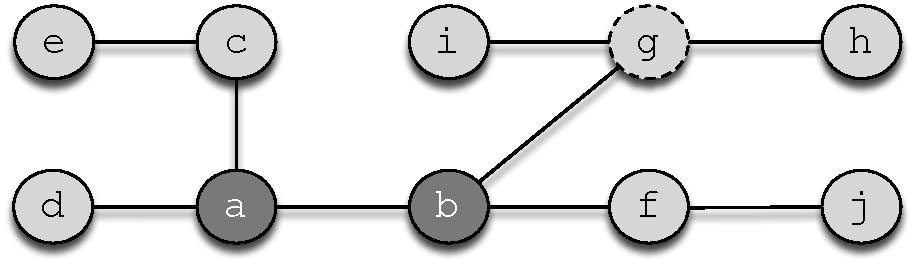
\includegraphics[scale=0.51]{figs/example4.pdf}
%\includegraphics[scale=0.51]{figs/example2.pdf}
\caption{Example power system graph. PMU nodes ($a,b$) are indicated with darker shading. Injection nodes have solid borders while zero-injection nodes  ($g$) have dashed borders.}
\label{fig:example}
\end{figure}

Using the same notation as Brueni and Heath \cite{Brueni05}, we define two $\Gamma$ functions. For $v\in V$ let $\Gamma(v)$ be the set of $v$'s neighbors in $G$, and $\Gamma[v] = \Gamma(v)\cup \{v\}$. 
% Since neighbor relationships are symmetric, $u\in\Gamma(v)\Rightleftarrow v\in\Gamma(u)$. 
A PMU placement $\Phi_G \subseteq V$ is a set of nodes at which PMUs are placed,
%We use the definition of a PMU placement from Brueni and Heath \cite{Brueni05}: a PMU cover, $\Phi$, is a subset of $V$ in which PMUs are placed such that all $v \in V$ and all $(u,v) \in E$ observed.
and $\Phi^R_G\subseteq V$ is the set of observed nodes for graph $G$ with placement $\Phi_G$ (see definition of observability below). %For convenience, we let $\Phi^R$ represent the observed nodes for graph $G$.
$k^* = \min \{|\Phi_G|:\Phi^R_G=V\}$ is used to denote the minimum number of PMUs needed to observe the entire network. Where the graph $G$ is clear from the context, we shall drop the $G$ subscript.
%Finally, $m$ is a constant corresponding to a graph $G=(V,E)$ such that $m < |V|$. 

%We let $\Phi^-$ represent the observed edges and $\Phi^R$ represent the observed nodes.
%All notation used in this document is shown in Table \ref{tab:notation}.

For convenience, we refer to any node with a PMU as a \emph{PMU node}. Additionally, for a given PMU placement we shall say that a set $W\subseteq V$ is observed if all nodes in the set are observed, and if $W=V$ we refer to the graph as \emph{fully observed}. 


%%%%%%%%%%%%%%%%%%%%%%%%%%%%%%%%%%%%%%%%%%%%%%%%%%%%%%%%%%%%%%%%%%%% BEGIN COMMENT %%%%%%%%%%%%%%%%%%%%%%%%%%%%%%%%%%%%%%%%%%%%%%%%%%%%%%%%%%%%%%%%%%%%%%%%%%%%%%%%%%%%%%%%%%%%%%%%%%%%%%%%%%%%%%%%
\begin{comment}
\begin{table}[t]
\begin{center}
\begin{tabular}{l l} 
\hline \hline
   	{\bf Notation} & {\bf Meaning} \\
		  \hline 
		  	$G$ &  undirected graph $(V,E)$ where each $v \in V$ is a bus and each \\
				&  $(u,v) \in E$ is a transmission line connecting $u$ and $v$\\
			$\Gamma(v)$ & $\{u \in V$ $|$ $(u,v) \in E \}$ \\ 
			$\Gamma[v]$ & $\Gamma(v) \cup \{v\}$ \\
 		 	$n$ & $|V|$ \\
			$\Phi$ & a subset of $V$ in which PMUs are placed such that all \\ 
				   & $v \in V$ and all $(u,v) \in E$ observed  \\
			$\Phi^R$ & set of observed nodes \\
			$\Phi^-$ & set of observed edges \\
			\hline \hline
	\end{tabular}
	\end{center}
\caption{Notation Table}
\label{tab:notation}
\end{table}
\end{comment}
%%%%%%%%%%%%%%%%%%%%%%%%%%%%%%%%%%%%%%%%%%%%%%%%%%%%%%%%%%%%%%%%%%%% END COMMENT %%%%%%%%%%%%%%%%%%%%%%%%%%%%%%%%%%%%%%%%%%%%%%%%%%%%%%%%%%%%%%%%%%%%%%%%%%%%%%%%%%%%%%%%%%%%%%%%%%%%%%%%%%%%%%%%

\subsection{Observability Rules}
\label{subsec:observe}

We use the simplified observability rules elegantly stated by Brueni and Heath \cite{Brueni05}. For completeness, we restate the rules here:
\begin{enumerate}
	
	\item {\bf Observability Rule 1 (O1)}.  {\it If node $v$ is a PMU node, then $\Gamma[v]$ is observed. Formally, if $v \in \Phi_G$, then $\Gamma[v] \subseteq \Phi^R_G$. }

	\item {\bf Observability Rule 2 (O2)}. {\it If a zero-injection node, $v$, is observed and  $\Gamma(v)\backslash\{u\}$ is observed for some $u\in\Gamma(v)$, then  $\Gamma[v]$ is observed.
	Formally, if $v \in \Phi^R_G \cap V_Z$ and $|\Gamma(v) \cap (V - \Phi^R_G)| \leq 1$, then $\Gamma[v] \subseteq \Phi^R_G$. }

\end{enumerate}

Consider the example in Figure \ref{fig:example}, where the shaded nodes are PMU nodes and $g$ is the only zero-injection node. 
%{\footnote {\small For all power system graphs shown in this document zero-injection nodes have a dashed border and injection nodes have a solid border.}}
Nodes $a-d$ are observed by applying O1 at the PMU at $a$, and nodes $a,b,f$ and $g$ are observed by applying O1 at $b$. 
$e$ cannot be observed via $c$ because $c$ does not have a PMU (O1 does not apply) and is an injection node (O2 does not apply). % so $e$ cannot be observed via $c$, which is its only neighbor. 
%$c$ does not have a PMU (O1 does not apply) and is an injection node (O2 does not apply), so $e$ cannot be observed via $c$, which is its only neighbor. 
Similarly, $j$ is not observed via $f$. Finally, although $g \in V_Z$, O2 cannot be applied at $g$ because $g$ has two unobserved neighbors $i,h$, so they remain unobserved.

Since O2 only applies with zero-injection nodes, more nodes might be observed when nodes are zero-injection. For example, consider the case where $c$ and $f$ are {\em zero-injection} nodes. $a-d$, $g$ and $f$ are still observed as before, as O1 makes not conditions on the node type. Additionally, 
since now $c,f \in V_Z$ and each has a single unobserved neighbor,  we can apply O2 at each of them to observe $e,j$, respectively. % making $e$ and $j$, respectively, observed.   
We evaluate the effect of increasing the number of zero-injection nodes on observability in our simulations (Section \ref{subsec:zero}).

%Finally, O2 can be applied at $e$ because $e \in V_Z$, $e$ is observed, and all of $e$'s neighbors except $i$ are observed. As a result, $i$ becomes observed. 
%Note that O2 cannot be applied at $f$ because $f$ has two unobserved neighbors. %This leaves $g$ and $h$ as the only two unobserved nodes in this example. 

%\begin{figure*}[t]
%  \begin{center}
%    \fbox{\subfigure[Case O1]{\label{fig:s1}\includegraphics[scale=0.28]{figs/s1.pdf}}}
%    \fbox{\subfigure[Case O2]{\label{fig:s2}\includegraphics[scale=0.28]{figs/s2.pdf}}} 
%  \end{center}
%	\caption{Rule Set 2} 
%  \label{fig:ruleset2}
%\end{figure*}




\subsection{Cross-Validation Rules}
\label{subsec:xval-rules}

% If phasor measured by 2 or more PMUs
From Vanfretti et al. \cite{Vanfretti10}, PMU measurements can be cross-validated when: (1) a 
voltage phasor of a non-PMU bus can be computed by PMU data from two different buses or (2) the current phasor of a transmission line can be computed from PMU data from two different buses. 
%Note that Vanfretti et al. \cite{Vanfretti10} use the term ``redundancy'' instead of cross-validation.  
{\footnote {\small  Vanfretti et al. \cite{Vanfretti10} use the term ``redundancy'' instead of cross-validation. }}  
Although it is the PMU data that is actually being cross-validated,
for convenience, we say a PMU is cross-validated. 
A PMU is \emph{cross-validated} if one of the rules below is satisfied\cite{Vanfretti10}: 
\begin{enumerate}
	
	\item {\bf Cross-Validation Rule 1 (XV1)}.  {\it If two PMU nodes are adjacent, then the PMUs cross-validate each other. % (Figure \ref{fig:validate}(a)). 
	Formally, if $u, v \in \Phi_G$, $u \in \Gamma(v)$, then the PMUs at $u$ and $v$ are cross-validated.}

	\item {\bf Cross-Validation Rule 2 (XV2)}. {\it If two PMU nodes have a common neighbor, then the PMUs cross-validate each other. % (Figure \ref{fig:validate}(b)). 
	Formally, if $u, v \in \Phi_G$, $u\neq v$ and $\Gamma(u)\cap\Gamma(v)=\emptyset$, then the PMUs at $u$ and $v$ are cross-validated.}
\end{enumerate}
In short, the cross-validation rules require that {\em the PMU is within two hops of another PMU}.
For example, in Figure \ref{fig:example}, the PMUs at $a$ and $b$ cross-validate each other by XV1. 
XV1 derives from the fact that both PMUs are measuring the current phasor of the transmission line connecting the two PMU nodes.  XV2 is more subtle.  
Using the notation specified in XV2, when computing the voltage phasor of an element in $\Gamma(u)\cap\Gamma(v)$ the equations include variables to account for measurement error (e.g., angle bias).
%In order to account for measurement error, the equations used to compute the voltage phasor of the neighbor node shared by the PMU nodes include varialbes to account
%for measurement error. Computing the voltage phasor of the neighbor node shared by the two PMU nodes
%When computing the voltage phasor of the common neighbor node shared by the PMU nodes the equations include variables to account for measurement error (e.g., angle bias). 
When the PMUs are two hops from each other, there are more equations than unknowns, allowing for measurement error detection. 
Otherwise, the number of unknown variables exceeds the number of equations, which eliminates the possibility of detecting measurement errors \cite{Vanfretti-thesis}.
%Otherwise, the number of unknown variables grows faster than the number of equations, which eliminates the possibility of detecting measurement errors \cite{Vanfretti-thesis}.




